\documentclass[ngerman,compress]{beamer}

\mode<presentation>
{
  \useoutertheme[footline=titleinstituteauthor]{c4}
  \useinnertheme{circles}
  \usecolortheme{c4}
  %\setbeamercovered{transparent}
  \setbeamercovered{highly dynamic}
}

\usepackage{babel}
\usepackage[utf8]{luainputenc}
\usepackage{fontspec}
\usepackage{listings}
\usepackage{color}

% Multimedia
%\usepackage{multimedia}

% sets the listings style
\definecolor{sh_comment}{rgb}{0.12, 0.38, 0.18 } %adjusted, in Eclipse: {0.25, 0.42, 0.30 } = #3F6A4D
\definecolor{sh_keyword}{rgb}{0.3, 0.3, 0.875}  % #5F1441
\definecolor{sh_string}{rgb}{0.875, 0.85, 0.11} % #101AF9

\lstset{basicstyle=\tiny\ttfamily,
	showspaces=false,
	showtabs=false, 
	showstringspaces=false, 
	columns=fullflexible, 
	stringstyle=\color{sh_string},
	keywordstyle=\color{sh_keyword}\bfseries,
	commentstyle=\color{sh_comment}\itshape
	}

\title[Hello, World! - u23 2012]
{\textbf{Hello, World!}\\u23 2013}

\author[andy <andy@koeln.ccc.de>]
{andy, florob, gordin, ike, meise, tobix, zakx}

\institute[Chaos Computer Club Cologne]
{
Chaos Computer Club Cologne e.V.\\
http://koeln.ccc.de \\
}

\date{Cologne\\2013-10-21}

\pgfdeclareimage[height=1cm]{barcode}{./c4-logo}
\logo{\pgfuseimage{barcode}}


% Folgendes sollte gelC6scht werden, wenn man nicht am Anfang jedes
% Unterabschnitts die Gliederung nochmal sehen möchte.
%\AtBeginSection[]
%{
%  \begin{frame}<beamer>
%    \frametitle{Gliederung}
%    \tableofcontents[currentsection,currentsubsection]
%  \end{frame}
%}

% Falls Aufzählungen immer schrittweise gezeigt werden sollen, kann
% folgendes Kommando benutzt werden:
%\beamerdefaultoverlayspecification{<+->}


\begin{document}

\begin{frame}
  \titlepage
\end{frame}

\AtBeginSubsection

\begin{frame}
  \tableofcontents
  % Die Option [pausesections] könnte nützlich sein.
\end{frame}


\section{Einführung}

\subsection{Zeitplan}
\begin{frame}
	%\frametitle{Erfa-Kreise}
	\begin{itemize}
		\item Einführung
		\begin{itemize}
			\item 2013-10-19 11:00 --- C99 Einführung (heute)
		\end{itemize}
		\item Reguläre Termine
		\begin{itemize}
			\item 2013-10-21 19:30 --- STM32-Einführung
			\item 2013-10-28 19:30 --- Peripherie des STM32
			\item 2013-11-04 19:30 --- Kommunikation mit anderen Bausteinen
			\item 2013-11-11 19:30 --- Kommunikation mit anderen Bausteinen (2)
			\item 2013-11-18 19:30 --- Projektarbeit
			\item 2013-11-25 19:30 --- Projektarbeit
			\item 2013-11-28 19:30 --- OpenChaos
		\end{itemize}
	\end{itemize}
\end{frame}

\subsection{Hardware}

\begin{frame}
	\frametitle{STM32F4 Discovery}
		\begin{columns}
			\column{1.5in}
				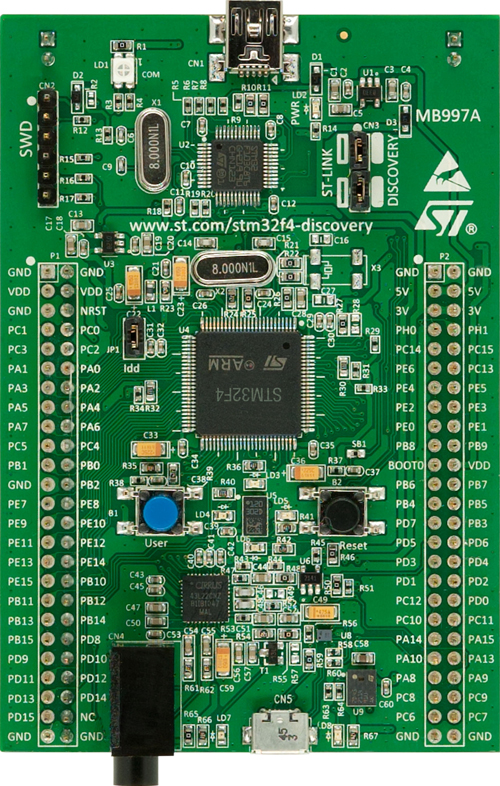
\includegraphics[height=2in]{stm32f4_discovery.jpg}
			\column{1.5in}
				\begin{itemize}
				\item STM32F407VGT6 32-bit ARM Cortex-M4F
				\item 1 MB Flash 
				\item 192 KB RAM (64KB CCM, 128KB SRAM)
				\item JTAG via ST-Linkv2
				\item USB OTG
				\item 100pin LQFP
				\end{itemize}
		\end{columns}
\end{frame}

\begin{frame}
	\frametitle{Boarddetails}
	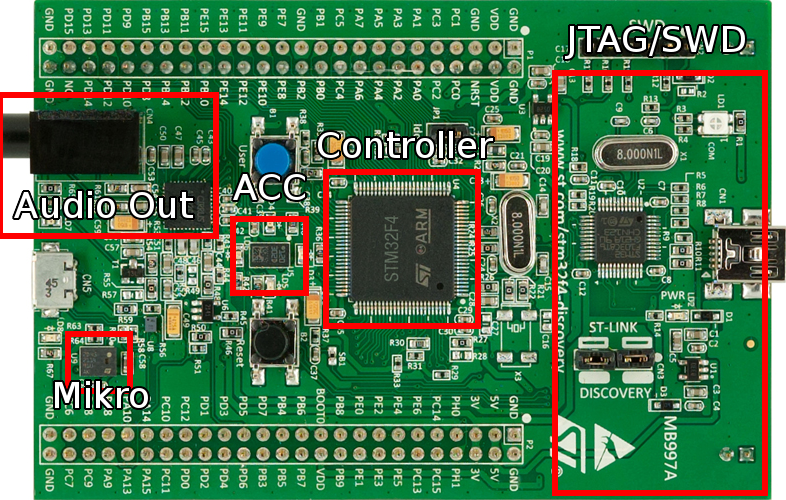
\includegraphics[height=2.5in]{stm32f4_discovery_beschriftet.png}
\end{frame}

\begin{frame}
	\frametitle{STM32F407}
	\begin{itemize}
		\item SoC = System on a Chip
		\item Lauffähiges Rechensystem komplett in einem Chip
		\item Nicht nur CPU + RAM, auch andere Peripherie:
		\begin{itemize}
			\item USARTs
			\item SPI-Controller
			\item I2C-Controller
			\item DCMI-(Kamera) Controller
			\item DMA-Engines
			\item GPIOs
			\item USB-Controller
			\item ... (siehe Datasheets später)
		\end{itemize}
		Bei nem "richtigen" PC ist oberer Kram alles im Chipsatz
	\end{itemize}
\end{frame}

\begin{frame}
	\frametitle{Chipübersicht}
	Datasheets sind eure Freunde! Ihr müsst allerdings auch erstmal lernen, wie man sie liest.
	\begin{itemize}
		\item Blockdiagramm: Datasheet STM32F407xx Seite 18
		\item Alternate Pin Functions: Datasheet STM32F407xx Seite 45
		\item Memory Map: Datasheet STM32F407xx Seite 63
	\end{itemize}
	Ist leider alles zu groß für die Slides :( \\
	Datasheets liegen im Libarary-Repo unter docs/
\end{frame}


\begin{frame}
	\frametitle{Externe Peripherie}
	Wir haben einiges an externen Bauteilen bestellt. China sollte irgendwann liefern.
	\begin{itemize}
		\item Servos
		\item Character- und (ein) Grafikdisplay
		\item Funkmodule
		\item Real-time clocks
		\item SD-Kartenadapter
		\item Magnetometer
		\item Ultraschall Entfernungssensoren
		\item 7-Segmentanzeigen
		\item Breadboards
		\item Kabel zum \$stuff zusammenstecken
		\item LEDs
		\item Buttons/Joysticks
	\end{itemize}
\end{frame}

\begin{frame}
	\frametitle{Projekte}
	Am Ende sollt ihr mit diesen Bausteinen was hübsches bauen. \\
	Erste Idee (vllt. etwas übertrieben): 3D-Scanner
	\begin{itemize}
		\item Zu scannendes Objekt sitzt auf einem Drehteller
		\item Ultraschall-Entfernungsmesser misst Entfernung zum Objekt
		\item Objekt wird etwas gedreht, nochmal gemessen
		\item Wenn eine Zeile fertig ist, Sensor in nächste Zeile schieben
		\item Irgendwann hat man dann vielleicht ein gescanntes 3D-Objekt
	\end{itemize}
	Sowas in der Art, gerne auch einfacher. Seid kreativ!
\end{frame}


\section{Chaos}

\subsection{Erfas}

\begin{frame}
	\frametitle{Erfas}
	\begin{itemize}
		\item Es gibt einen großen bundesweiten CCC e.V.
		\item Und viele kleine lokale CCCs wie den C4
		\item Unterscheidung zwischen Erfas und Chaostreffs
		\item Beides sind Lokalitäten mit (meist) eigenen Räumen
		\item Dienen als Treffpunkt für Hacker und Häcksen in einer Stadt
	\end{itemize}
\end{frame}


\begin{frame}
	\frametitle{C4}
	\begin{itemize}
		\item Der C4 hat seit Ewigkeiten Erfastatus
		\item Seit gut zwei Jahren haben wir größere Räume
		\item Auszug unserer Projekte
		\begin{itemize}
			\item Frab (Konferenzverwaltungssystem)
			\item CCC Kassensystem
			\item Jährliches U23
			\item media.ccc.de
			\item Seit kurzem Teile des VOCs
			\item (und diverse eigene Projekte der Mitglieder)
		\end{itemize}
	\end{itemize}
\end{frame}


\begin{frame}
	\frametitle{Congress}
	\begin{itemize}
		\item Bald ist der Chaos Communication Congress (30C3) in Hamburg
		\item Findet vom 27.12. bis 30.12. statt
		\item Sollte euch der Kram hier interessieren, fahrt da mal hin!
		\item C4 wird ein Assembly haben, ihr kennt da also dann auch schon Leute :)
	\end{itemize}
\end{frame}
